\documentclass[11pt]{article}
\usepackage[utf8]{inputenc} % Para caracteres en espa�ol
\usepackage{amsmath,amsthm,amsfonts,amssymb,amscd}
\usepackage{multirow,booktabs}
\usepackage[table]{xcolor}
\usepackage{fullpage}
\usepackage{lastpage}
\usepackage{enumitem}
\usepackage{multicol}
\usepackage{fancyhdr}
\usepackage{mathrsfs}
\usepackage{pdfpages}
\usepackage{wrapfig}
\usepackage{setspace}
\usepackage{esvect}
\usepackage{calc}
\usepackage{multicol}
\usepackage{cancel}
\usepackage{graphicx}
\graphicspath{ {} }
\usepackage[retainorgcmds]{IEEEtrantools}
\usepackage[margin=3cm]{geometry}
\usepackage{amsmath}
\newlength{\tabcont}
\setlength{\parindent}{0.0in}
\setlength{\parskip}{0.05in}
\usepackage{empheq}
\usepackage{framed}
\usepackage[most]{tcolorbox}
\usepackage{xcolor}
\colorlet{shadecolor}{orange!15}
\parindent 0in
\parskip 12pt
\geometry{margin=1in, headsep=0.25in}
\theoremstyle{definition}
\newtheorem{defn}{Definition}
\newtheorem{reg}{Rule}
\newtheorem{exer}{Exercise}

% Two more packages that make it easy to show MATLAB code
\usepackage[T1]{fontenc}
\usepackage[framed,numbered]{matlab-prettifier}
\lstset{
	style = Matlab-editor,
	basicstyle=\mlttfamily\small,
}

\begin{document}
\begin{center}
\begin{lstlisting}
function hw7clean
    l = 0.05; % Channel Length [m]
    %Constant Density
    tMaxCD = 4.69e-6;
    tspan = linspace(0, tMaxCD,100);
    [tCD,xx] = ode23s(@snowplowi,tspan,[0.00001,0]);
    xCD = xx(:,1);
    xdotCD = xx(:,2);
    
    %Linearly Decreasing Density
    tMaxLDD = 3.8311e-6;
    tspan = linspace(0, tMaxLDD, 100);
    [tLDD,xx] = ode23s(@snowplowii,tspan,[0.00001,0]);
    xLDD = xx(:,1);
    xdotLDD = xx(:,2);
    
    %Square Root Dependence,Decreasing Density 
    tMaxSQD = 4.19633e-6;
    tspan = linspace(0, tMaxSQD,100);
    [tSQD,xx] = ode23s(@snowplowiii,tspan,[0.00001;0]);
    xSQD = xx(:,1);
    xdotSQD = xx(:,2);
    
    %Note: Plotting code removed for space
end

function xdot = snowplowi(t,x)
    l = 0.05; area = 0.03*0.03; R_A = 208.13; P_o = 66.661185; T_o = 273; rho = P_o / (R_A * T_o);J = 20e3; Lprime = 0.6E-6; F = 0.5*Lprime*J^2; 
    m = area*rho*x(1);
    mdot = area*rho*x(2);
    xdot = [x(2); (F-(mdot*x(2)))/m];
end

function xdot = snowplowii(t,x)
    l = 0.05; area = 0.03*0.03; R_A = 208.13; P_o = 66.661185; T_o = 273; rho = P_o / (R_A * T_o);J = 20e3; Lprime = 0.6E-6; F = 0.5*Lprime*J^2; 
    m = area*rho*(x(1)-(((x(1))^2)/(2*l)));
    mdot = area*rho*x(2)*(1-(x(1)/l));
    xddot = F\[mdot m]
    xdot = [x(2); (F-(mdot*x(2)))/m]
end

function xdot = snowplowiii(t,x)
    l = 0.05; area = 0.03*0.03; R_A = 208.13; P_o = 66.661185; T_o = 273; rho = P_o / (R_A * T_o);J = 20e3; Lprime = 0.6E-6; F = 0.5*Lprime*J^2; 
    m = area*rho*(-(2/3)*(l - x(1))*sqrt(1 - x(1)/l)+((2/3)*l)); 
    mdot = area*rho*sqrt(1-(x(1)/l))*x(2);
    xdot = [x(2); (F-(mdot*x(2)))/m];
end
\end{lstlisting}
\newpage
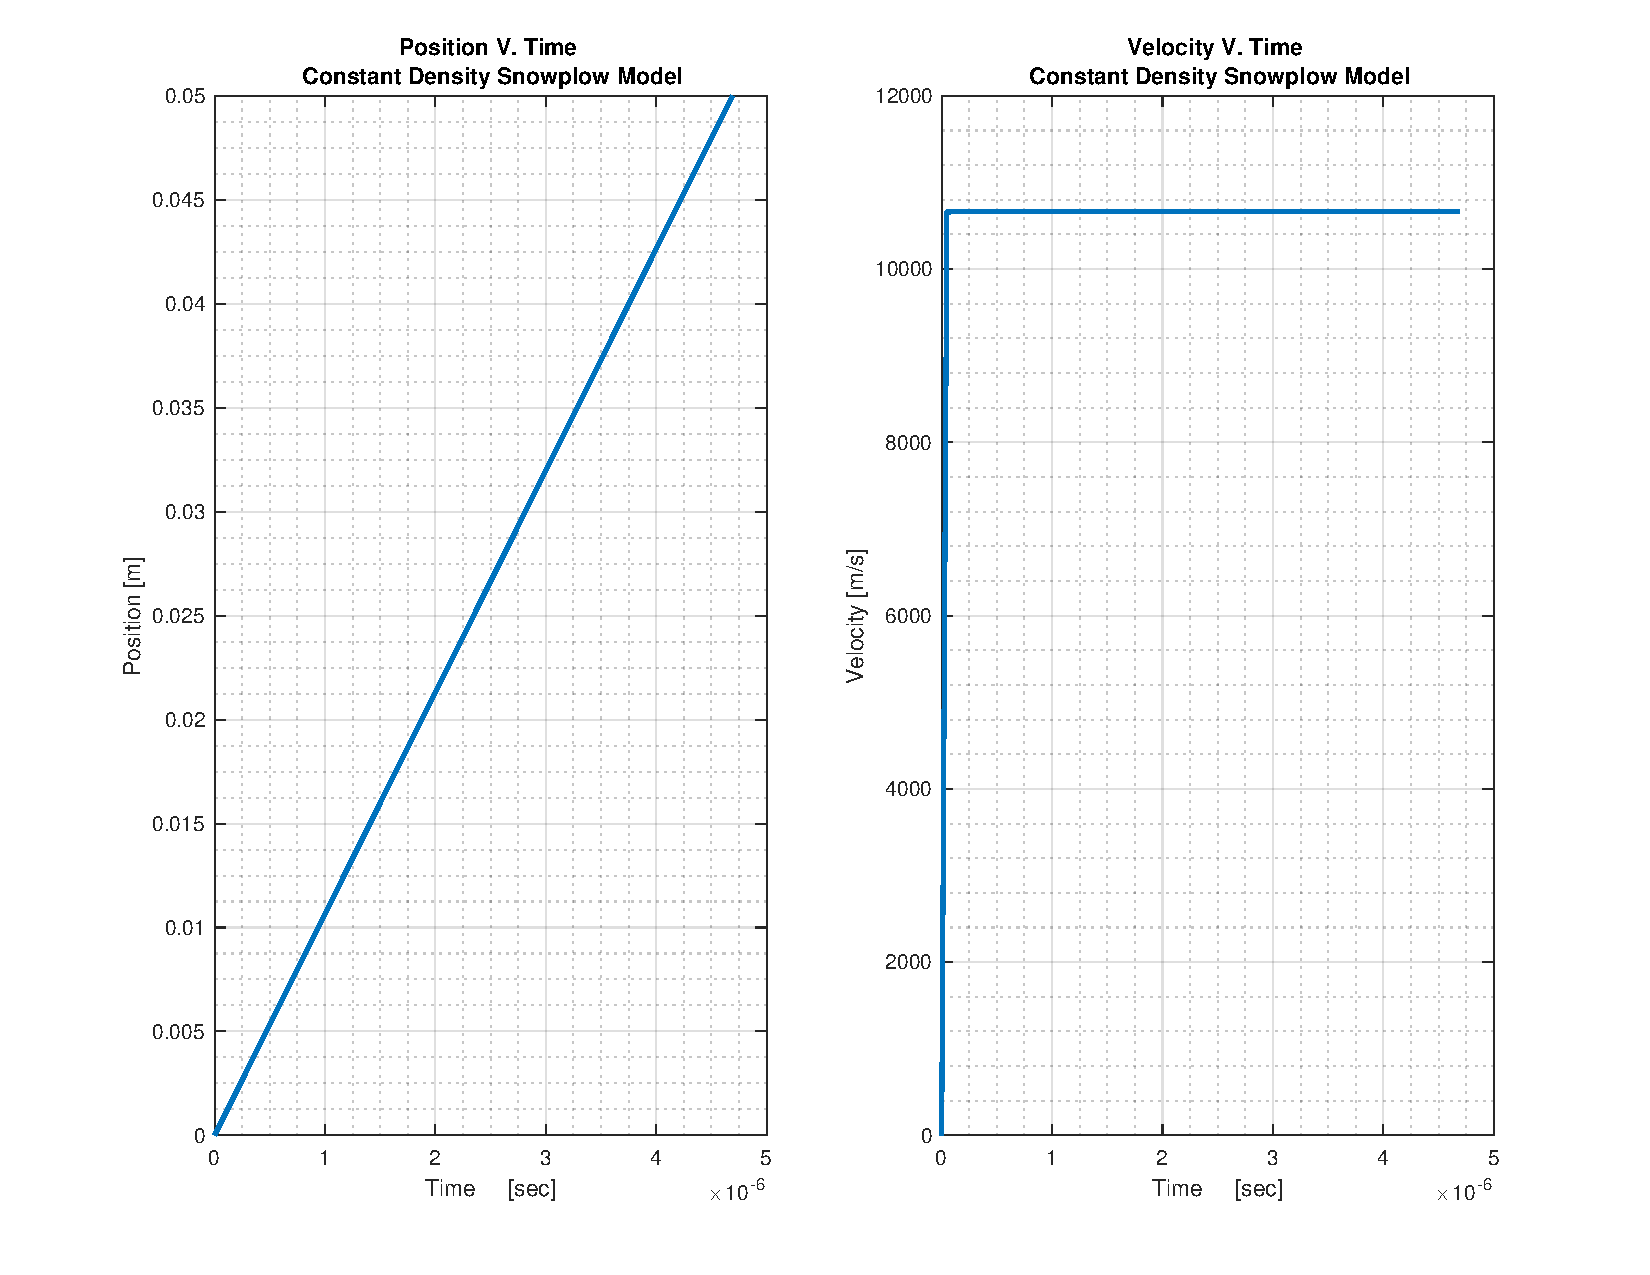
\includepdf[landscape=true]{Problem2PartCi.pdf}
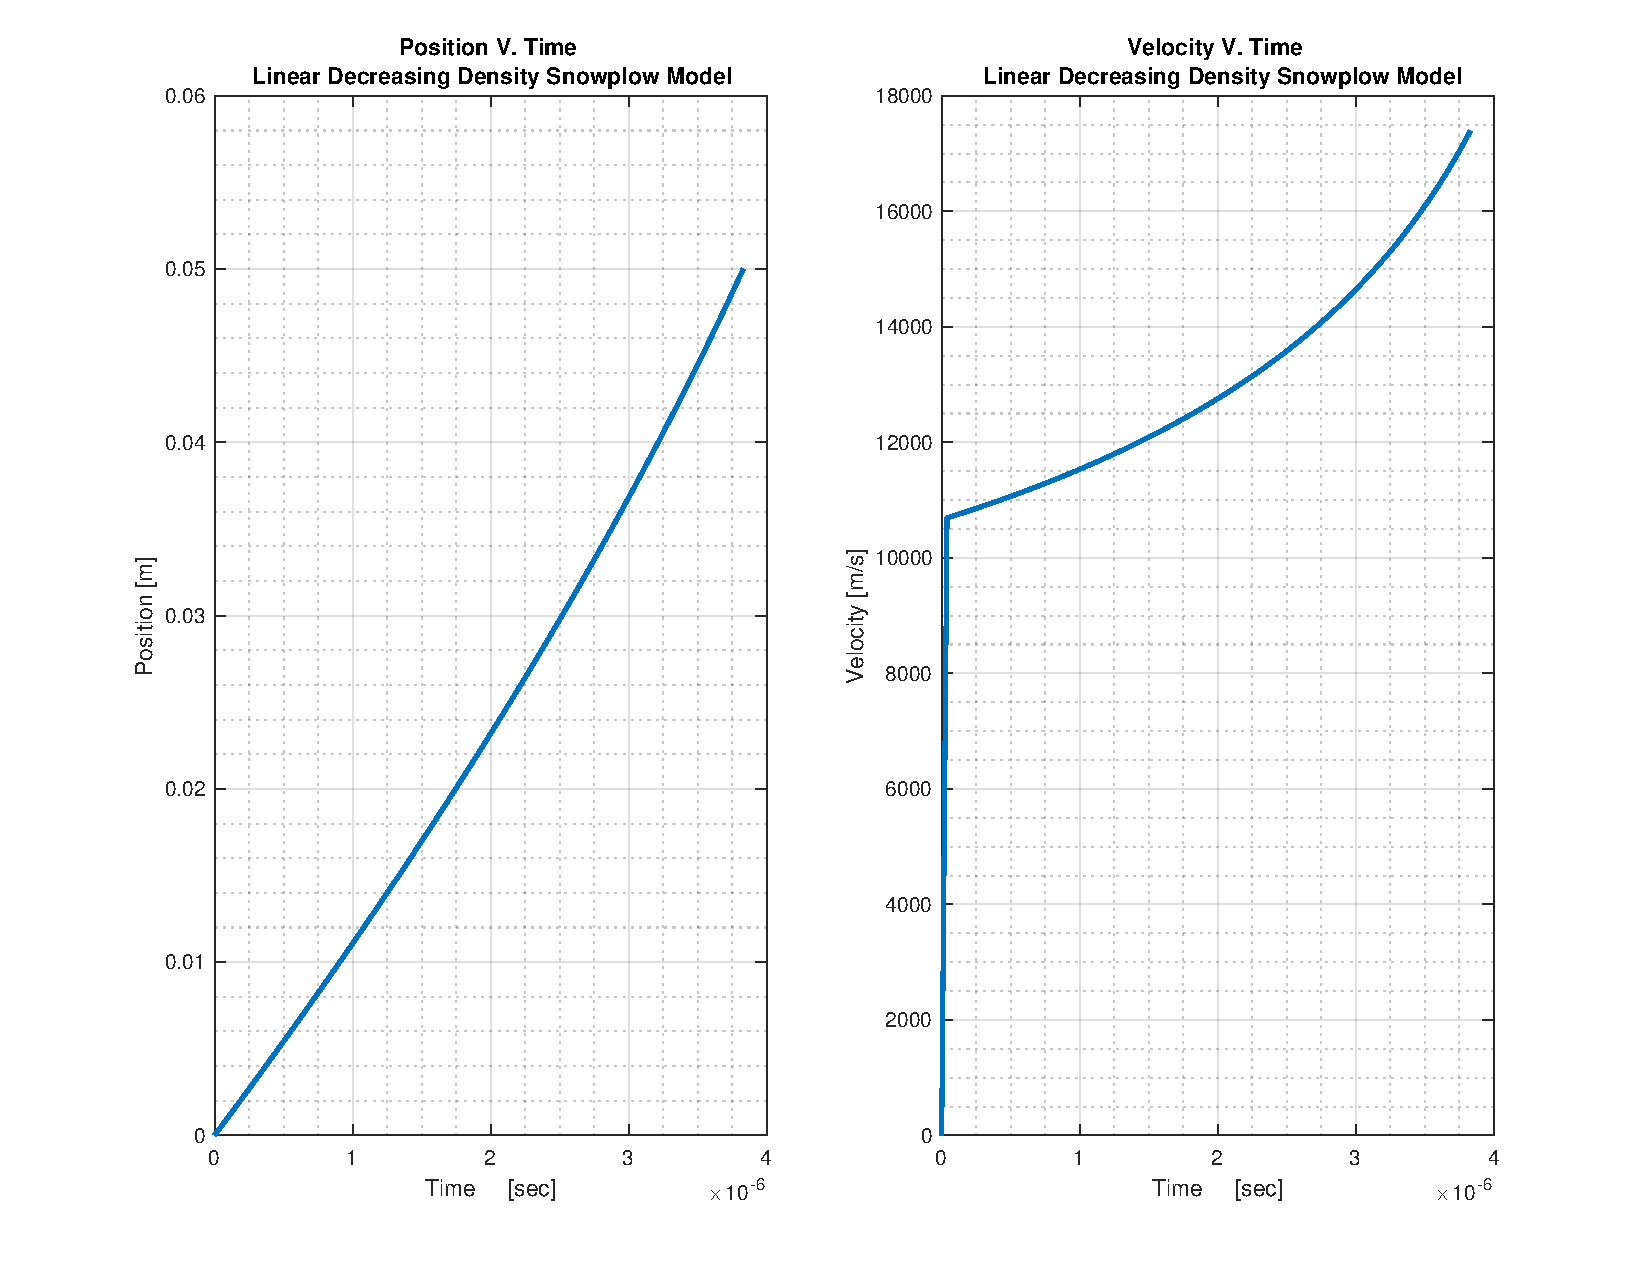
\includepdf[landscape=true]{Problem2PartCii.pdf}
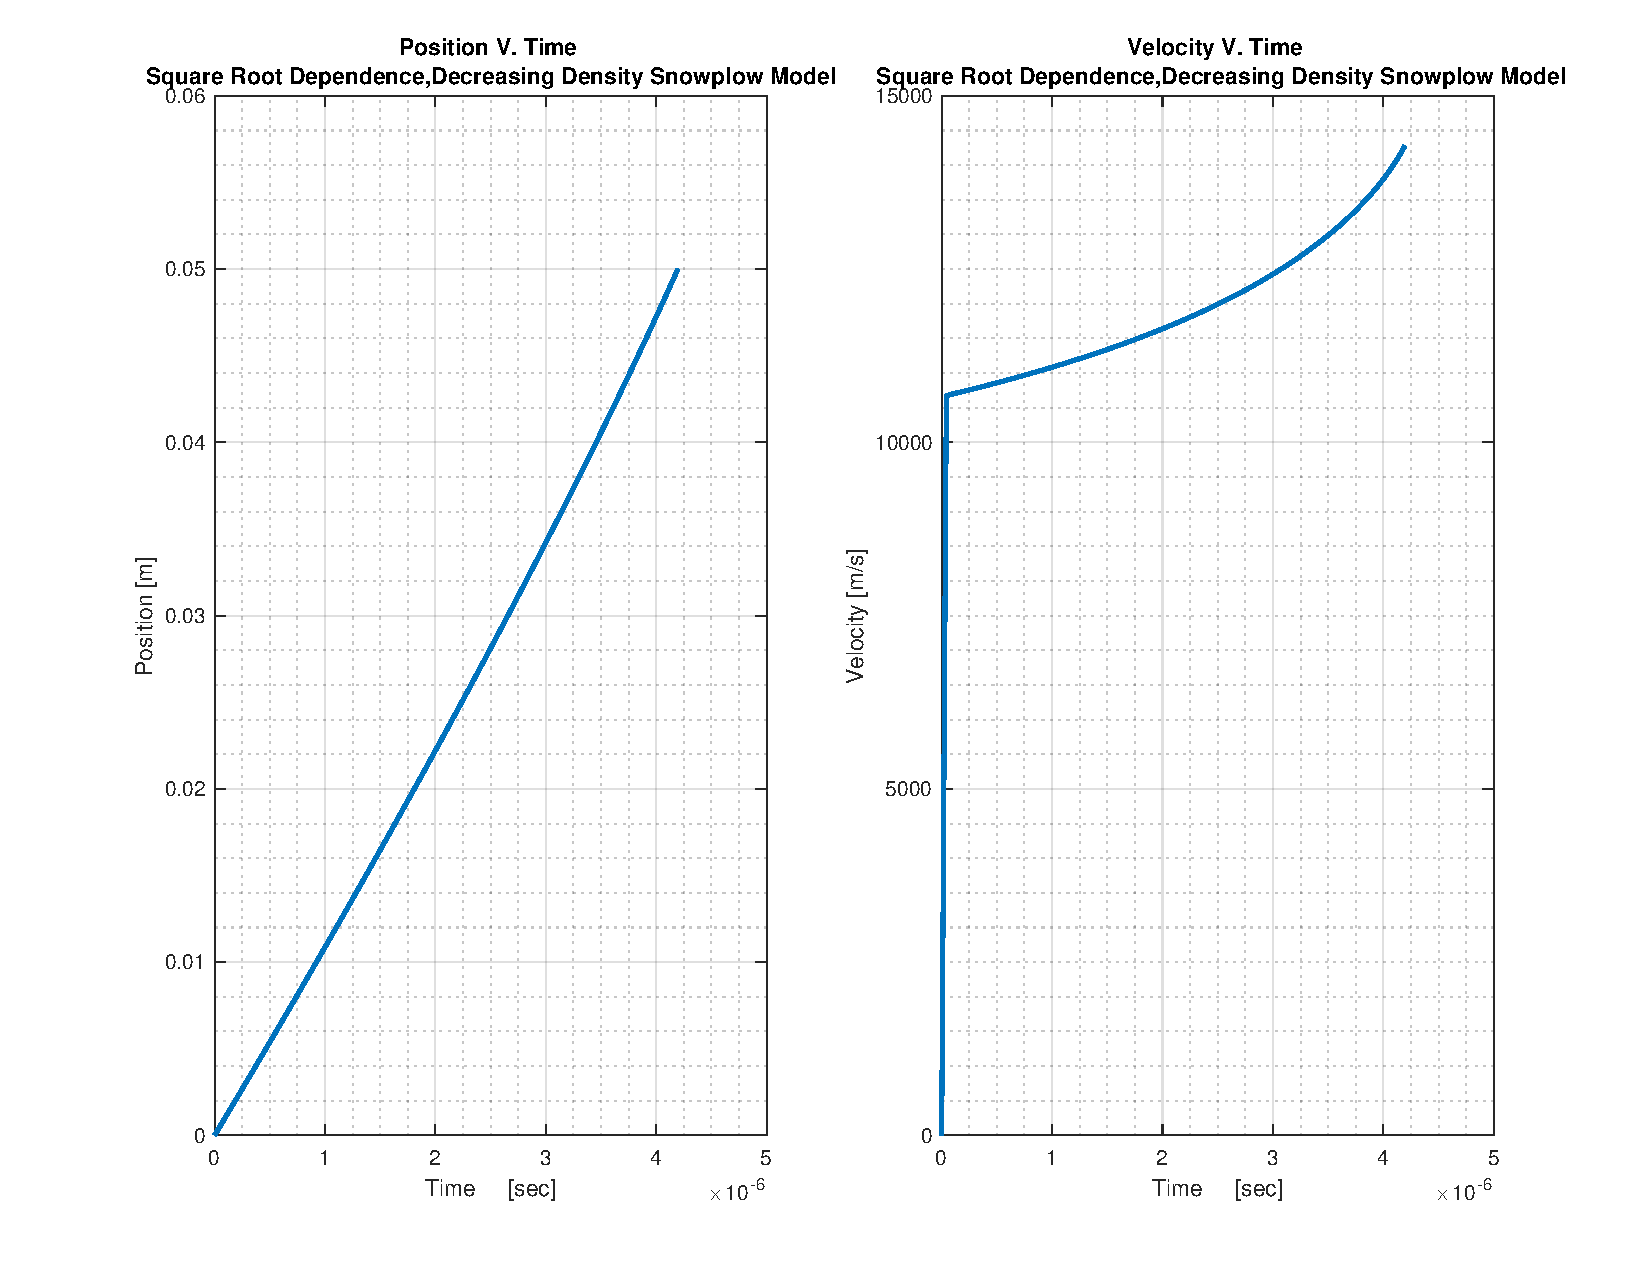
\includepdf[landscape=true]{Problem2PartCiii.pdf}
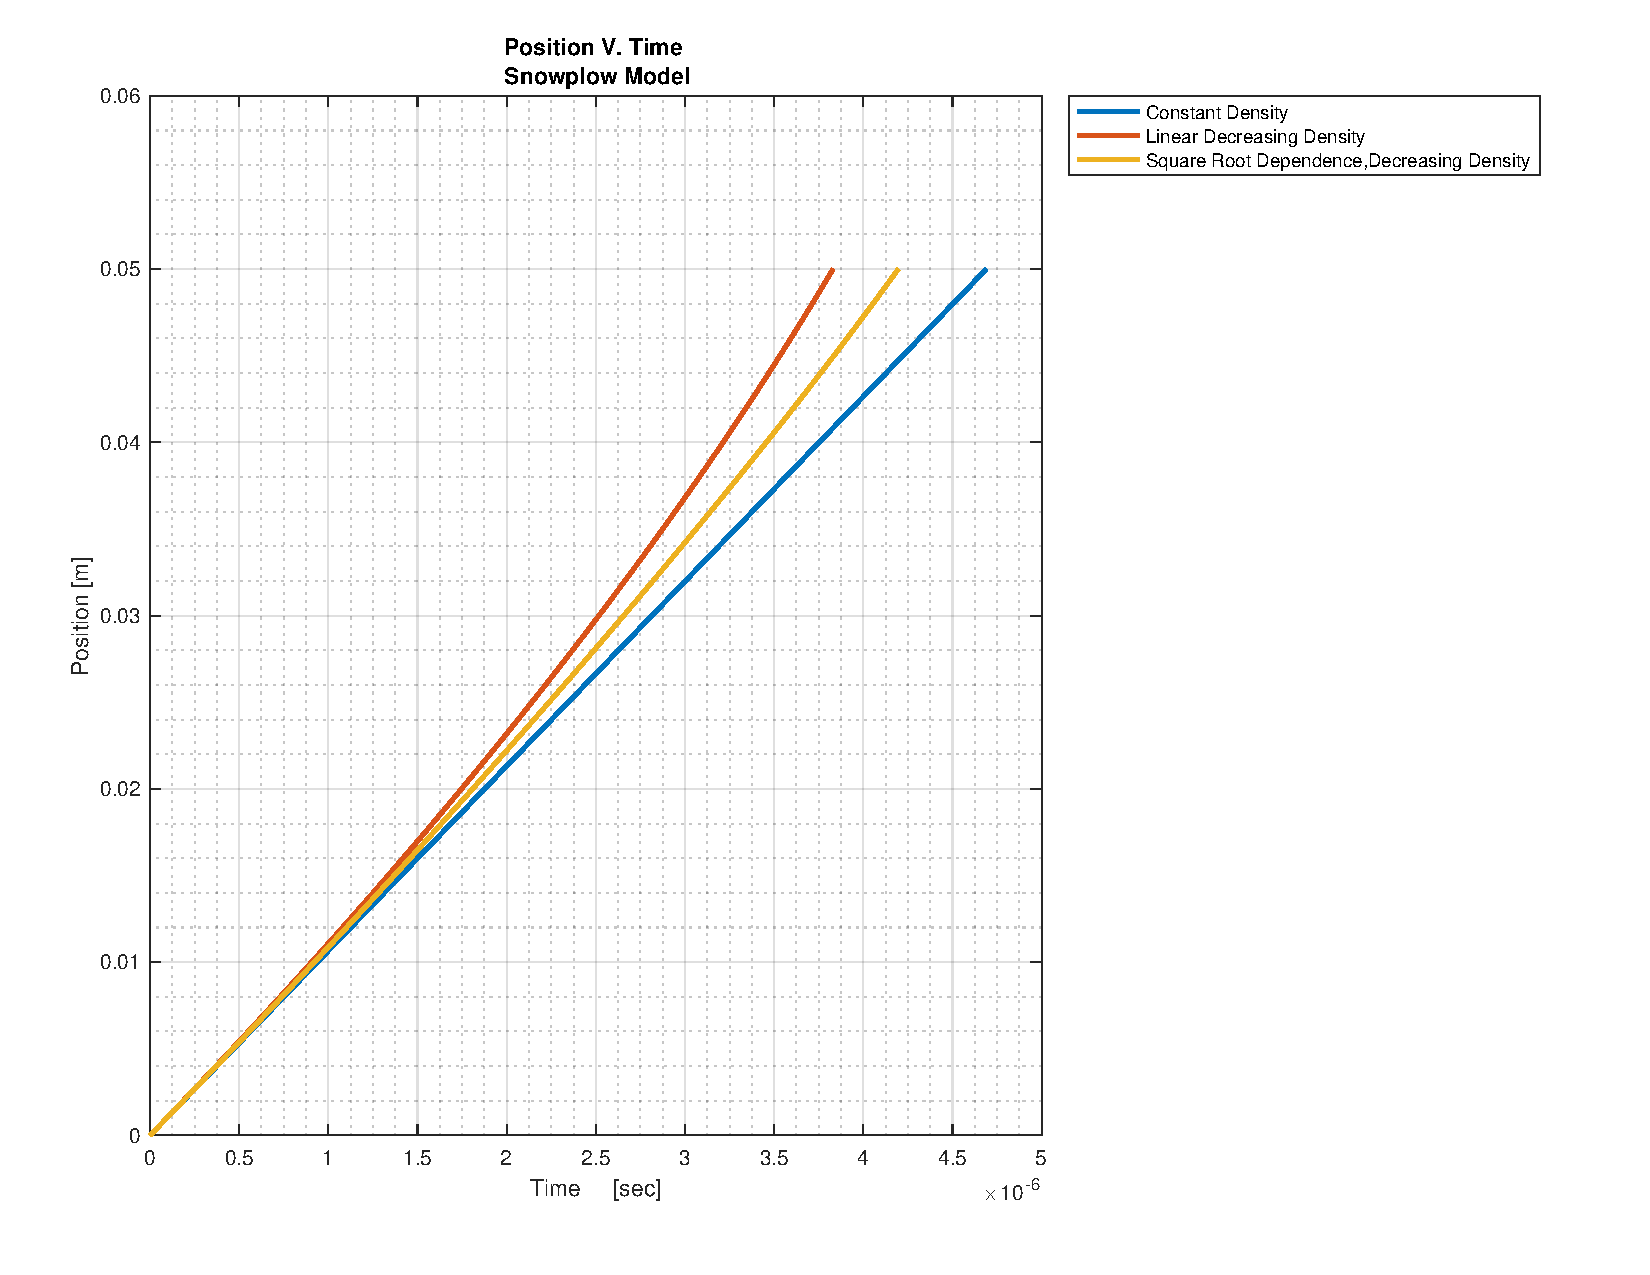
\includepdf[landscape=true]{Problem2PartD.pdf}
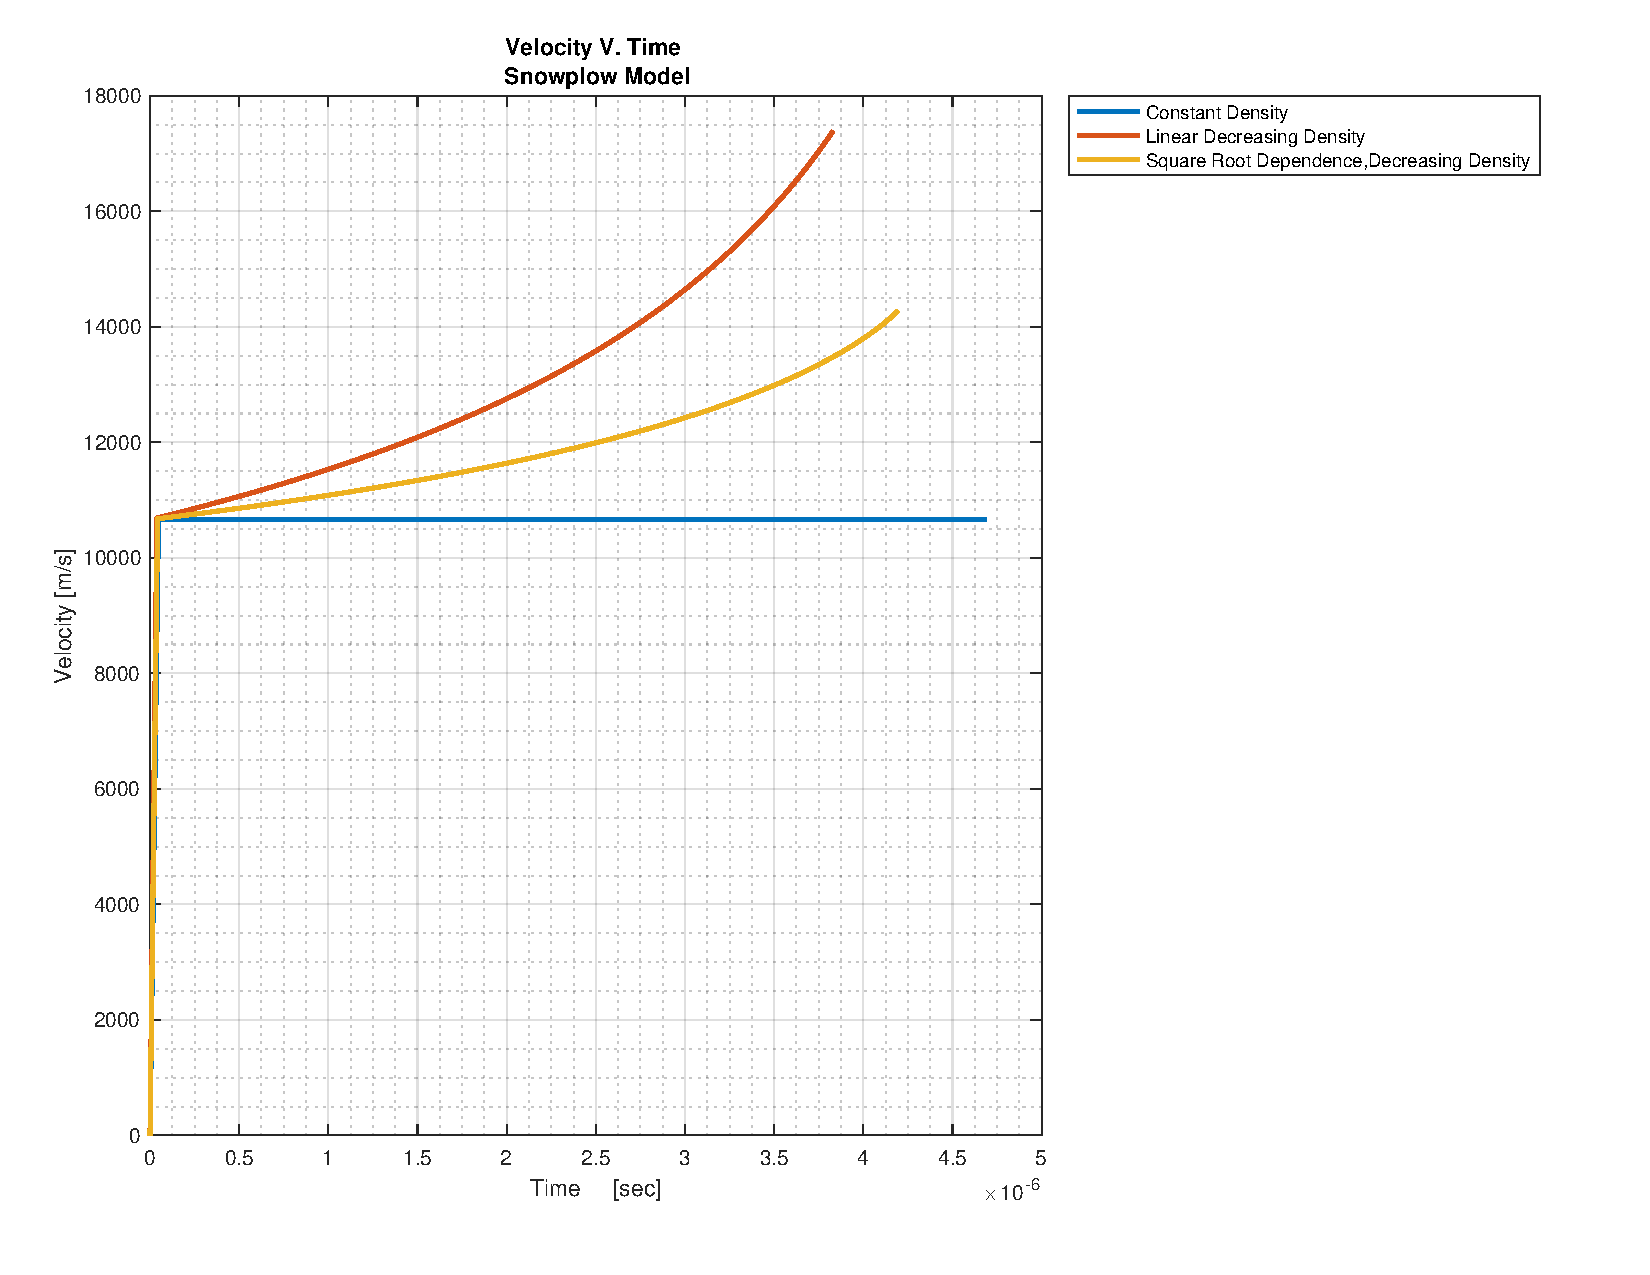
\includepdf[landscape=true]{Problem2PartE.pdf}
\end{document}